\documentclass[reqno, 12pt]{amsart}

\usepackage{amssymb, amsmath, amsthm, enumerate, mathtools, graphicx, enumitem, tikz, color, soul, bbm, verbatim, parskip, multicol}
\usepackage[margin=1 in]{geometry}
\usepackage[mathscr]{euscript}
\usepackage[urlcolor=blue,colorlinks=true]{hyperref}
\setlist[itemize]{noitemsep, topsep=0pt, parsep=0pt, partopsep=0pt}
\allowdisplaybreaks

\newcommand{\R}{\mathbb R}
\newcommand{\proj}{\operatorname{proj}}
%%%%%%%%%%%%%%%%%%%%%%%%%%%%%%%%%%%%%
\usepackage{mdframed}
\newmdenv[
  linewidth=1pt,
  linecolor=black,
  topline=true,
  bottomline=true,
  leftline=true,
  rightline=true,
  innertopmargin=10pt,
  innerbottommargin=10pt,
  innerleftmargin=10pt,
  innerrightmargin=10pt
]{answerbox}

\usepackage{pgfplots}
\pgfplotsset{compat=1.18}
\usepgfplotslibrary{fillbetween}
%%%%%%%%%%%%%%%%%%%%%%%%%%%%%%%%%%%%%

\pagestyle{plain}


\begin{document}

\begin{center}
  {\bf MATH 231-01: Homework Assignment 10}\\~\\
  2 December 2025\\~\\~\\~\\~\\~\\
\end{center}

{\bf Due:} 9 December 2025 by 10:00pm Eastern time, submitted on Moodle as a single PDF.~\\


{\bf Instructions:} Write your solutions on the following pages. If you need more space, you may add pages, but make sure they are in order and label the problem number(s) clearly. You should attempt each problem on scrap paper first, before writing your solution here. Excessively messy or illegible work will not be graded. You must show your work/reasoning to receive credit. You do not need to include every minute detail; however the process by which you reached your answer should be evident. You may work with other students, but please write your solutions in your own words.

~\\~\\~\\~\\~\\
{\bf Name:} Sean Balbale

~\\
{\bf Score:}

\newpage
\begin{itemize}

  \item[1.] Let $\Sigma$ be the surface parametrized by
    \begin{align*}
      {\bf r}(s,t) = \langle (2+\cos t)\cos s, (2+\cos t)\sin s, \sin t\rangle, \quad\quad s,t \in [0,2\pi].
    \end{align*}
    Use GeoGebra (or another online tool) to visualize $\Sigma$, then find its surface area. (Hint: If ${\bf u},{\bf v} \in \R^3$ and ${\bf u} \cdot {\bf v} = 0$, then $\|{\bf u}\times{\bf v}\| = \|{\bf u}\|\|{\bf v}\|$.)
    \newline

    \begin{answerbox}
      \begin{center}
        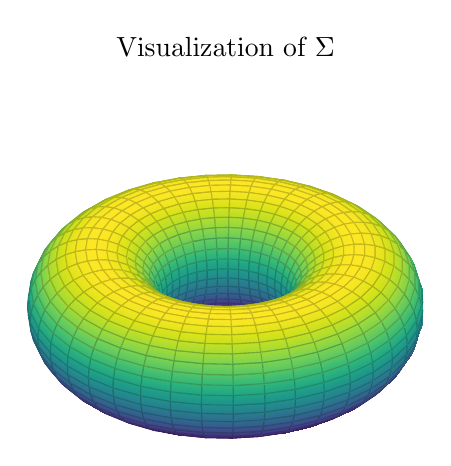
\begin{tikzpicture}
          \begin{axis}[
              title={Visualization of $\Sigma$},
              axis equal,
              hide axis,
              view={60}{30},
              colormap/viridis,
            ]
            \addplot3[
              surf,
              shader=faceted interp,
              samples=40,
              samples y=40,
              domain=0:360,
              domain y=0:360,
              z buffer=sort
            ]
            (
              {(2 + cos(y)) * cos(x)}, % x component
              {(2 + cos(y)) * sin(x)}, % y component
              {sin(y)}                 % z component
            );
          \end{axis}
        \end{tikzpicture}

        \begin{enumerate}
          \item Compute ${\bf r}_s$ and ${\bf r}_t$:
            \[{\bf r}_s = \langle -(2+\cos t)\sin s, (2+\cos t)\cos s, 0 \rangle\]
            \[{\bf r}_t = \langle -\sin t \cos s, -\sin t \sin s, \cos t \rangle\]
          \item Compute the cross product ${\bf r}_s \times {\bf r}_t$:
            \[{\bf r}_s \times {\bf r}_t = \langle(2+\cos t)\cos s \cos t, (2+\cos t)\sin s \cos t, (2+\cos t)\sin t \rangle\]
          \item Compute the magnitude $\|{\bf r}_s \times {\bf r}_t\|$:
            \[\|{\bf r}_s \times {\bf r}_t\| = (2+\cos t)\sqrt{\cos^2 t + \sin^2 t} = (2+\cos t)\]
          \item Set up the surface area integral:
            \[A = \int_0^{2\pi} \int_0^{2\pi} (2+\cos t) \, ds \, dt\]
          \item Evaluate the integral:
            \[A = \int_0^{2\pi} \int_0^{2\pi} (2+\cos t) \, ds \, dt = \int_0^{2\pi} (2+\cos t)(2\pi) \, dt = 2\pi \int_0^{2\pi} (2+\cos t) \, dt\]
            \[= 2\pi \left[ 2t + \sin t \right]_0^{2\pi} = 2\pi (4\pi) = 8\pi^2\]
          \item Final answer:
            \[\boxed{8\pi^2}\]
        \end{enumerate}
      \end{center}



    \end{answerbox}
    \newpage
  \item[2.] Let $\Sigma$ be the surface parametrized by
    \begin{align*}
      {\bf r}(s,t) = \langle s\cos t, s \sin t, t\rangle, \quad\quad s \in [-1,1],~ t \in [0,2\pi].
    \end{align*}
    Use GeoGebra (or another online tool) to visualize $\Sigma$, then write down an iterated integral whose value is the surface area of $\Sigma$. (You do not need to evaluate the integral, but you can try to do so as a challenge, or look it up.)
    \newline

    \begin{answerbox}
      \begin{center}

        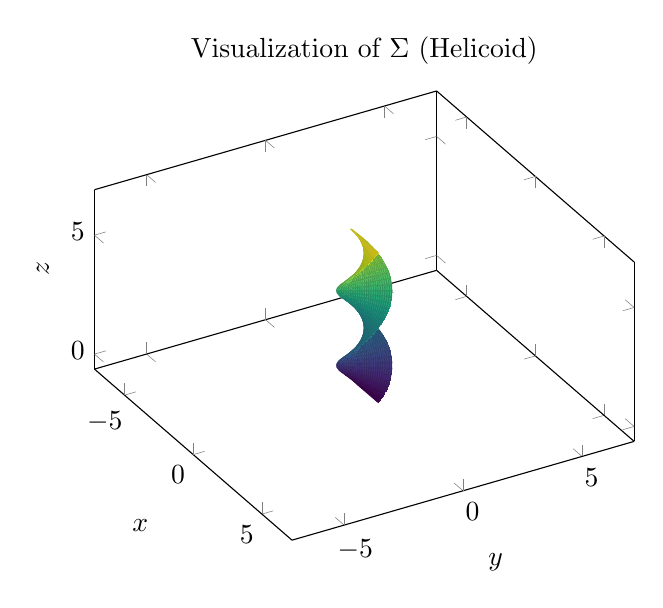
\begin{tikzpicture}
          \begin{axis}[
              title={Visualization of $\Sigma$ (Helicoid)},
              axis equal,
              view={60}{30},
              xlabel=$x$, ylabel=$y$, zlabel=$z$,
              colormap/viridis,
            ]
            \addplot3[
              surf,
              shader=faceted interp,
              samples=25,       % Adjust for resolution
              samples y=40,
              domain=-1:1,      % Domain for s
              domain y=0:360,   % Domain for t (degrees)
              z buffer=sort
            ]
            (
              {x * cos(y)},     % x = s * cos(t)
              {x * sin(y)},     % y = s * sin(t)
              {y*pi/180}        % z = t (converted to radians for height scaling)
            );
          \end{axis}
        \end{tikzpicture}
      \end{center}

      \begin{enumerate}
        \item Compute ${\bf r}_s$ and ${\bf r}_t$:
          \[{\bf r}_s = \langle \cos t, \sin t, 0 \rangle\]
          \[{\bf r}_t = \langle -s \sin t, s \cos t, 1 \rangle\]
        \item Compute the cross product ${\bf r}_s \times {\bf r}_t$:
          \[{\bf r}_s \times {\bf r}_t = \langle \sin t, -\cos t, s \rangle\]
        \item Compute the magnitude $\|{\bf r}_s \times {\bf r}_t\|$:
          \[\|{\bf r}_s \times {\bf r}_t\| = \sqrt{\sin^2 t + \cos^2 t + s^2} = \sqrt{1 + s^2}\]
        \item Set up the surface area integral:
          \[A = \int_0^{2\pi} \int_{-1}^{1} \sqrt{1 + s^2} \, ds \, dt\]
        \item Final answer:
          \[\boxed{\int_0^{2\pi} \int_{-1}^{1} \sqrt{1 + s^2} \, ds \, dt}\]

      \end{enumerate}
    \end{answerbox}


    \newpage
  \item[3.] Let $\Sigma$ be the part of the cone $z = \sqrt{x^2+y^2}$ that lies between the planes $z=1$ and $z=2$, oriented with upward/inward unit normal vector. Calculate the flux of ${\bf F}(x,y,z) = \langle x,y,z\rangle$ through $\Sigma$.
    \newline

    \begin{answerbox}
      \begin{enumerate}
        \item Parametrize the surface using cylindrical coordinates:
          \[{\bf r}(r,\theta) = \langle r\cos\theta, r\sin\theta, r \rangle, \quad r \in [1,2], \theta \in [0,2\pi]\]
        \item Compute ${\bf r}_r$ and ${\bf r}_\theta$:
          \[{\bf r}_r = \langle \cos\theta, \sin\theta, 1 \rangle\]
          \[{\bf r}_\theta = \langle -r\sin\theta, r\cos\theta, 0 \rangle\]
        \item Compute the cross product ${\bf r}_r \times {\bf r}_\theta$:
          \[{\bf r}_r \times {\bf r}_\theta = \langle -r\cos\theta, -r\sin\theta, r \rangle\]
        \item Compute the magnitude $\|{\bf r}_r \times {\bf r}_\theta\|$:
          \[\|{\bf r}_r \times {\bf r}_\theta\| = r\sqrt{2}\]
        \item Set up the flux integral:
          \[\Phi = \int_0^{2\pi} \int_1^{2} {\bf F}({\bf r}(r,\theta)) \cdot \frac{{\bf r}_r \times {\bf r}_\theta}{\|{\bf r}_r \times {\bf r}_\theta\|} \|{\bf r}_r \times {\bf r}_\theta\| \, dr \, d\theta\]
        \item Evaluate the integral:
          \[\Phi = \int_0^{2\pi} \int_1^{2} \langle r\cos\theta, r\sin\theta, r \rangle \cdot \langle -\cos\theta, -\sin\theta, 1 \rangle r\sqrt{2} \, dr \, d\theta\]
          \[= \int_0^{2\pi} \int_1^{2} ( -r^2 + r^2 ) \sqrt{2} \, dr \, d\theta = 0\]
        \item Final answer:
          \[\boxed{0}\]
      \end{enumerate}
    \end{answerbox}
    \newpage
  \item[4.] Let $C$ be the curve parametrized by
    \begin{align*}
      {\bf r}(t) = \langle \cos(t)^3, \sin(t)^3\rangle, \quad\quad t \in [0,2\pi],
    \end{align*}
    and let $R$ be the region enclosed by $C$. Use GeoGebra (or another online tool) to visualize $R$, then find the area of $R$ by applying Green's theorem. (Hint: Use the vector field ${\bf F}(x,y) = \frac{1}{2}\langle-y,x\rangle$. The identity $\sin(t)^2\cos(t)^2 = \frac{1}{8}(1-\cos(4t))$ will be helpful.)
    \newline

    \begin{answerbox}

      \begin{enumerate}
        \item Set up the area integral using Green's theorem:
          \[A = \oint_C {\bf F} \cdot d{\bf r} = \iint_R \left( \frac{\partial Q}{\partial x} - \frac{\partial P}{\partial y} \right) dA\]
          where ${\bf F}(x,y) = \frac{1}{2}\langle -y, x \rangle$, so $P = -\frac{y}{2}$ and $Q = \frac{x}{2}$.
        \item Compute the partial derivatives:
          \[\frac{\partial Q}{\partial x} = \frac{1}{2}, \quad \frac{\partial P}{\partial y} = -\frac{1}{2}\]
        \item Substitute into the area integral:
          \[A = \iint_R (1) dA\]
        \item Parametrize the curve $C$:
          \[x(t) = \cos^3 t, \quad y(t) = \sin^3 t, \quad t \in [0, 2\pi]\]
        \item Compute $dx$ and $dy$:
          \[dx = -3\cos^2 t \sin t dt, \quad dy = 3\sin^2 t \cos t dt\]
        \item Set up the line integral:
          \[A = \int_0^{2\pi} {\bf F}({\bf r}(t)) \cdot {\bf r}'(t) dt\]
          where ${\bf r}'(t) = \langle -3\cos^2 t \sin t, 3\sin^2 t \cos t \rangle$.
        \item Evaluate the line integral:
          \[A = \int_0^{2\pi} \frac{1}{2} \langle -\sin^3 t, \cos^3 t \rangle \cdot \langle -3\cos^2 t \sin t, 3\sin^2 t \cos t \rangle dt\]
          \[= \int_0^{2\pi} \frac{1}{2} (3\sin^4 t \cos^2 t + 3\cos^4 t \sin^2 t) dt\]
          \[= \frac{3}{2} \int_0^{2\pi} \sin^2 t \cos^2 t dt\]
          \[= \frac{3}{16} \left[ t - \frac{\sin(4t)}{4} \right]_0^{2\pi} = \frac{3}{16} (2\pi) = \frac{3\pi}{8}\]
        \item Final answer:
          \[\boxed{\frac{3\pi}{8}}\]
      \end{enumerate}
    \end{answerbox}

    \newpage
  \item[5.] Let $C$ be the curve within the surface $z = 2+\cos x + \sin y$ that lies directly above the square with vertices $(0,0),(0,\pi),(\pi,0),(\pi,\pi)$ and is oriented counterclockwise when viewed from above. Let ${\bf F}(x,y,z) = \langle z-3y,x+z,2y\rangle$. Evaluate
    \begin{align*}
      \int_C {\bf F}\cdot d{\bf r}.
    \end{align*}
    \newline

    \begin{answerbox}
      \begin{enumerate}
        \item By Stokes' Theorem: $\int_C {\bf F} \cdot d{\bf r} = \iint_S (\nabla \times {\bf F}) \cdot d{\bf S}$.
        \item Calculate Curl(${\bf F}$):
          \[\nabla \times {\bf F} =
            \begin{vmatrix} {\bf i} & {\bf j} & {\bf k} \\ \partial_x & \partial_y & \partial_z \\ z-3y & x+z & 2y
          \end{vmatrix}\]
          \[= {\bf i}(2 - 1) - {\bf j}(0 - 1) + {\bf k}(1 - (-3)) = \langle 1, 1, 4 \rangle\]
        \item Find the normal vector ${\bf n} \, dS$:
          For surface $z = 2+\cos x+\sin y$, oriented upward (consistent with counterclockwise $C$):
          \[{\bf n} \, dS = \langle -z_x, -z_y, 1 \rangle \, dA\]
          \[z_x = -\sin x, \quad z_y = \cos y\]
          \[{\bf n} \, dS = \langle \sin x, -\cos y, 1 \rangle \, dA\]
        \item Evaluate the dot product:
          \[(\nabla \times {\bf F}) \cdot {\bf n} = \langle 1, 1, 4 \rangle \cdot \langle \sin x, -\cos y, 1 \rangle = \sin x - \cos y + 4\]
        \item Integrate over the region $[0,\pi] \times [0,\pi]$:
          \[\int_{0}^{\pi} \int_{0}^{\pi} (\sin x - \cos y + 4) \, dy \, dx\]
        \item Inner integral ($y$):
          \[[\sin x \cdot y - \sin y + 4y]_{0}^{\pi} = (\pi \sin x - 0 + 4\pi) - (0) = \pi \sin x + 4\pi\]
        \item Outer integral ($x$):
          \[\int_{0}^{\pi} (\pi \sin x + 4\pi) \, dx = [-\pi \cos x + 4\pi x]_{0}^{\pi}\]
          \[= (-\pi(-1) + 4\pi^2) - (-\pi(1) + 0) = \pi + 4\pi^2 + \pi = 2\pi + 4\pi^2\]
        \item Final answer:
          \[\boxed{2\pi + 4\pi^2}\]
      \end{enumerate}
    \end{answerbox}

    \newpage
  \item[6.] Let $\Sigma$ be the surface of the solid tetrahedron bounded by the planes
    \begin{align*}
      x=0, \quad y=0, \quad z=0, \quad x+y+z=1
    \end{align*}
    in the first octant, with outward unit normal vector ${\bf n}$. Let
    \begin{align*}
      {\bf F}(x,y,z) = \langle x^2+y, xy, -2xz-y\rangle.
    \end{align*}
    Evaluate
    \begin{align*}
      \int_\Sigma {\bf F}\cdot {\bf n}dS.
    \end{align*}
    \newline

    \begin{answerbox}
      \begin{enumerate}
        \item Compute the divergence of ${\bf F}$:
          \[\nabla \cdot {\bf F} = \frac{\partial (x^2 + y)}{\partial x} + \frac{\partial (xy)}{\partial y} + \frac{\partial (-2xz - y)}{\partial z}\]
          \[= 2x + x - 2x = x\]
        \item Set up the volume integral using the Divergence Theorem:
          \[\int_\Sigma {\bf F} \cdot {\bf n} dS = \iiint_V (\nabla \cdot {\bf F}) dV\]
          where $V$ is the tetrahedron bounded by the planes.
        \item Set up the limits of integration:
          \[0 \leq x \leq 1, \quad 0 \leq y \leq 1 - x, \quad 0 \leq z \leq 1 - x - y\]
        \item Evaluate the volume integral:
          \[\iiint_V x \, dz \, dy \, dx = \int_0^1 \int_0^{1-x} \int_0^{1-x-y} x \, dz \, dy \, dx\]
          \[= \int_0^1 \int_0^{1-x} x(1 - x - y) \, dy \, dx\]
          \[= \int_0^1 x\left[(1 - x)y - \frac{y^2}{2}\right]_0^{1-x} dx\]
          \[= \int_0^1 x\left[(1 - x)(1 - x) - \frac{(1 - x)^2}{2}\right] dx\]
          \[= \int_0^1 x\left[\frac{(1 - x)^2}{2}\right] dx = \frac{1}{2} \int_0^1 x(1 - 2x + x^2) dx\]
          \[= \frac{1}{2} \left[\frac{x^2}{2} - \frac{2x^3}{3} + \frac{x^4}{4}\right]_0^1 = \frac{1}{2} \left(\frac{1}{2} - \frac{2}{3} + \frac{1}{4}\right)\]
          \[= \frac{1}{2} \left(\frac{6 - 8 + 3}{12}\right) = \frac{1}{2} \cdot \frac{1}{12} = \frac{1}{24}\]
        \item Final answer:
          \[\boxed{\frac{1}{24}}\]
      \end{enumerate}
    \end{answerbox}
    \newpage
  \item[7.] Let $\Sigma$ be the surface of the solid region bounded by the cylinder $x^2+y^2=4$ and the planes $z=0$ and $z=3$, with outward unit normal vector ${\bf n}$. Let
    \begin{align*}
      {\bf F}(x,y,z) = \langle x^3,y^3,z^3\rangle.
    \end{align*}
    Evaluate
    \begin{align*}
      \int_\Sigma {\bf F}\cdot {\bf n}dS.
    \end{align*}
    \newline

    \begin{answerbox}
      \begin{enumerate}
        \item Compute the divergence of ${\bf F}$:
          \[\nabla \cdot {\bf F} = \frac{\partial (x^3)}{\partial x} + \frac{\partial (y^3)}{\partial y} + \frac{\partial (z^3)}{\partial z} = 3x^2 + 3y^2 + 3z^2\]
        \item Set up the volume integral using the Divergence Theorem:
          \[\int_\Sigma {\bf F} \cdot {\bf n} dS = \iiint_V (\nabla \cdot {\bf F}) dV\]
          where $V$ is the solid region bounded by the cylinder and planes.
        \item Convert to cylindrical coordinates:
          \[x = r\cos\theta, \quad y = r\sin\theta, \quad z = z\]
          \[dV = r \, dr \, d\theta \, dz\]
          The limits are: \(0 \leq r \leq 2\), \(0 \leq \theta \leq 2\pi\), \(0 \leq z \leq 3\).
        \item Evaluate the volume integral:
          \[\iiint_V (3r^2 + 3z^2) r \, dr \, d\theta \, dz = \int_0^{2\pi} \int_0^2 \int_0^3 (3r^3 + 3z^2 r) dz \, dr \, d\theta\]
          \[= \int_0^{2\pi} \int_0^2 [3r^3 z + r z^3]_0^3 dr d\theta = \int_0^{2\pi} \int_0^2 (9r^3 + 27r) dr d\theta\]
          \[= \int_0^{2\pi} [\frac{9r^4}{4} + \frac{27r^2}{2}]_0^2 d\theta = \int_0^{2\pi} (36 + 54) d\theta = 90 \int_0^{2\pi} d\theta = 90(2\pi) = 180\pi\]
        \item Final answer:
          \[\boxed{180\pi}\]
      \end{enumerate}
    \end{answerbox}
\end{itemize}
\end{document}
